\documentclass[conference]{IEEEtran}
\IEEEoverridecommandlockouts
% The preceding line is only needed to identify funding in the first footnote. If that is unneeded, please comment it out.
\usepackage{cite}
\usepackage{amsmath,amssymb,amsfonts}
\usepackage{algorithmic}
\usepackage{graphicx}
\usepackage{textcomp}
\usepackage{tikz}
\usepackage{tikzscale}
\usetikzlibrary{backgrounds,calc,decorations.pathreplacing,fit,matrix,patterns,positioning,shapes,shapes.multipart}
\def\BibTeX{{\rm B\kern-.05em{\sc i\kern-.025em b}\kern-.08em
    T\kern-.1667em\lower.7ex\hbox{E}\kern-.125emX}}
\begin{document}

\title{An Investigation into Stateless Blockchain}

\author{\IEEEauthorblockN{Student A}
\IEEEauthorblockA{Dept. of Computer Science \\
ID:12341000}
\and

\IEEEauthorblockN{Student B}
\IEEEauthorblockA{Dept. of Computer Science \\
ID:12341000}
\and

\IEEEauthorblockN{Student C}
\IEEEauthorblockA{Dept. of Computer Science \\
ID:12341000}
}

\maketitle


\section{Introduction}
Recent years have witnessed the prosperity of cryptocurrencies which seek for more efficient and secure financial
transactions through removing trusted third parties like escrows and banks~\cite{SongWP00}.
%
As their underlying technology, blockchain enables users to broadcast and confirm asynchronous transactions securely in an untrusted environment.
%
In order to achieve this, nodes in blockchain systems need to validate broadcasted transactions by querying the current system \textit{state}.
%
To be more specific, this state can be available by storing subsequent ordered blocks from the genesis block in local.

However, due to the ever-growing nature of the blockchain systems, the storage requirement is increasing linearly with the ledger length.
%
This restricted condition entails taking much storage space and time to download and maintain the entire history of blockchains.
%
For example, a new full node that wants to join in the Ethereum network and acquires the correct ledger \textit{state} needs to download 132.57 GB of data~\cite{Ethereumstorage} currently. 

As the emerging concerns on chain data size in the developer community, the concept of `stateless' blockchain has received considerable interests nowadays.
%
This concept is derived from a personal blog~\cite{delayed-txo-commitments}, which is proposed to avoid storing the whole state in an accumulative manner.
%
Unfortunately, realizing a blockchain system with lessened storage requirement is a quite difficult task due to many challenges.

For one thing, maintaining a public ledger in a decentralized system entails the duties of validating and broadcasting transaction on each node.
%
In order to check the validation of each transaction, nodes must store the current ledger \textit{state} that determines the ownership of existing assets.
%
For instance, the \textit{state} of Bitcoin is a data set of unspent transaction outputs (UTXOs). 
%
In order to check the validation of transactions, nodes should confirm that spent coin belongs to UTXO set locally.
%
In other words, nodes without storing UTXO set can't validate the incoming transactions.

For another thing, sharding or commitment schemes are viewed as effective methods to reduce the storage cost on each node.
%
In these ways, nodes could verify transactions by checking the membership proofs provided by issuers.
%
However, these solutions are actually at the cost of communication overhead across the system.
%
And high communication overhead would inevitably lead to the low scalability and throughput of the entire network, which is against the principles of cryptocurrencies.
%
How to leverage these tools to realize a cryptocurrency protocol is a challenging open question in blockchain community.

With these unresolved problems, I conduct an investigation into state-of-the-art solutions of stateless blockchain in this paper.
%
By categorizing existing literatures, I
%
I then pick up some important literatures and explain their algorithms in more detail.
%
By providing comprehensive evaluations for these methods, 

The rest of this paper is organized as follows: 


\begin{figure}[t]
  \centering
  \resizebox{0.7\linewidth}{!}{\begin{tikzpicture}[remember picture]
    \node (light-node){
        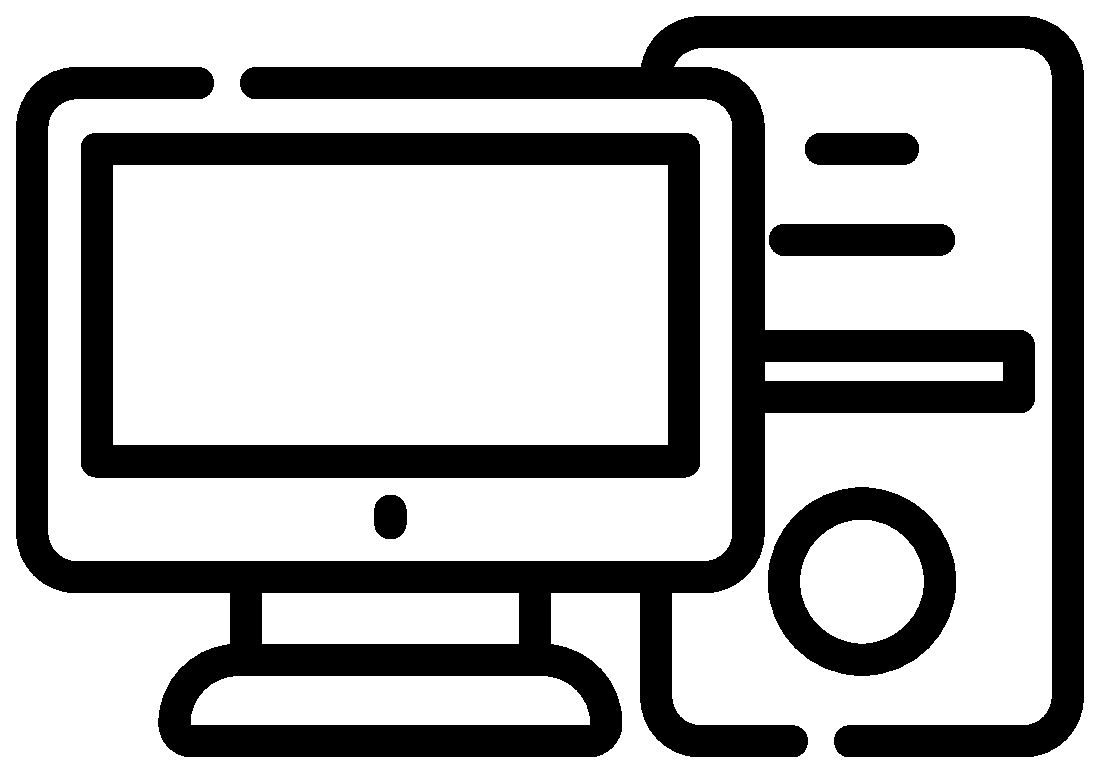
\includegraphics[scale = 0.05]{figs/icons/computer.eps}
    };
    \node[scale = 0.35,below=0cm of light-node] (light-label) {\textbf{Light Node}};

    \node (full-node) [matrix, below left = of light-node]{ 
        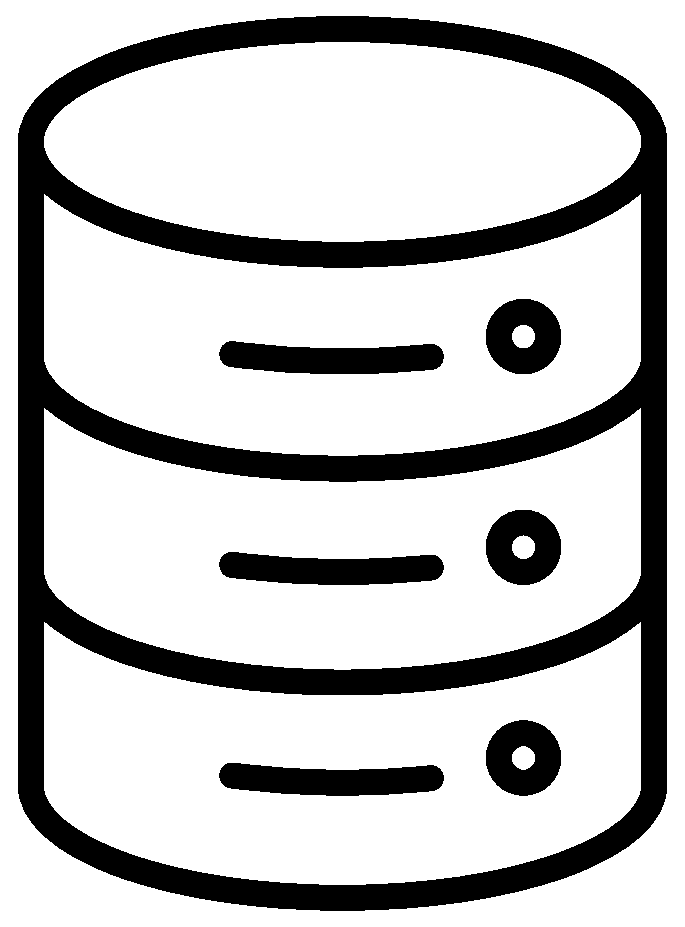
\includegraphics[scale = 0.05]{figs/icons/database.eps}
        \\
    };
    \node[scale = 0.35,below = 0cm of full-node,xshift=5ex] (full-label) {\textbf{Full Node}};

    \node (miner) [matrix, below right = 1.02cm and 0.5cm of light-node]{
        \includegraphics[scale = 0.45]{figs/icons/server.eps}
        \\
    };
    \node[scale = 0.35,below = 0cm of miner,xshift=6.5ex] (miner-label) {\textbf{Miner}};

    \draw [->] (-0.45,-0.05) -- (-1.3,-0.85) 
    node [above,midway,sloped,scale=0.3]
    {Query};

    \draw [<-] (-0.38,-0.17) -- (-1.15,-0.9) 
    node [below,midway,sloped,scale=0.3]
    {Answers \& Proof};

    \draw  (-1.15,-1.2) -- (1.2,-1.2);

    \draw [->] (0.45,-0.05) -- (1.35,-0.8) 
    node [above,midway,sloped,scale=0.3]
    {Query};

    \draw [<-] (0.42,-0.17) -- (1.22,-0.82) 
    node [below,midway,sloped,scale=0.3]
    {Answers \& Proof};
\end{tikzpicture}}
  \caption{System Architecture}\label{fig:model}
\end{figure}

\section{Application Setting}
\subsection{System Architecture}
In this subsection, I will briefly introduce the system architecture of current blockchains.
%
As shown in Figure, there exist three kinds of nodes with different functionalities in a classical blockchain network:
\textit{full nodes}, \textit{miners} and \textit{light nodes}.
%
To fulfill the security model, full nodes must download blocks originated from the first block all the way and validate them against consensus proof.
%
To be specific, a full node store all blocks including block headers and data records on the disk.
%
Miners are full nodes with high computational power, who could execute consensus protocol (e.g. hash puzzle in Bitcoin) and generate new blocks for money rewards.
%
Restricted in limited resources, a light node only needs to download block headers during the initial syncing process and then requests transactions from connected full nodes as needed.

\subsection{Stateless Blockchain}
In the current blockchain system, locally maintaining the validation state means quite cumbersome work. 
%
On one hand, this high storage requirement potentially fails those users who can't dedicate large storage space to join in the network.
%
More than that, increasing storage requirement might also reduce the incentives for running full nodes, which could lead to possible centralization of blockchains.
%
On the other hand, full nodes tend to leverage database (e.g. LevelDB in geth client) to manage the entire ledger \textit{state},
which causes expensive I/O costs and prolong the validation time.

Due to the above concerns, the blockchain community is eager for a well-designed protocol to tackle these issues by lessening or even removing local validation state.

%\begin{table}[h]
%\centering
%\caption{Comparison of encrypted search schemes.}
%\label{my-label}
%\begin{tabular}{|l|l|l|}
%\hline
%Scheme & Search Complexity & Index Size \\ \hline
%\cite{SongWP00}   & ...              & ...       \\ \hline
%...    & ...               & ...        \\ \hline
%\end{tabular}
%\end{table}

\section{Background on transaction validation in current blockchain systems}


\section{Research Directions of Stateless Blockchain}
%

Guidelines: In this subsection, you should introduce the typical research directions for encrypted search, describe in detail the goals of each research direction in terms of functionality and/or security. You should also specify and discuss the design challenges in each direction based on your literature study and or your personal perspectives. Besides, you should properly discuss the existing works and try to reflect the state-of-the-art. A possible organization structure is given below. 


%\begin{figure}[!t]
%  \centering
%  \includegraphics[width=2in]{./fig1.png}
%  \caption{Outsourcing encrypted data to the cloud.}
%  \label{fig_model}
%\end{figure}

\subsection{Basic Searchable Encryption}

\textbf{Goals.} The description goes here.


\textbf{Design challenges.} The description goes here.

\textbf{Related work.} The description goes here.

\subsection{Dynamic Searchable Encryption}

\textbf{Goals.} The description goes here.


\textbf{Design challenges.} The description goes here.

\textbf{Related work.} The description goes here.




\subsection{Boolean Searchable Encryption}

\textbf{Goals.} The description goes here.


\textbf{Design challenges.} The description goes here.

\textbf{Related work.} The description goes here.

\subsection{Any Other Possible Categories}

\textbf{Goals.} The description goes here.


\textbf{Design challenges.} The description goes here.

\textbf{Related work.} The description goes here.

\section{Conclusion}

The conclusion goes here.


\bibliographystyle{IEEEtran}
\bibliography{references}


\end{document}
